\chapter{Discussion}
\label{cha:discussion}


During the project we faced a lot of obstacles and some things which needed to be changed. In this chapter we discuss our design, the methods used, as well as discuss and highlight some of the problems we have faced, why they may have happened and how they could be fixed. We will also discuss what changes that were made and also what could have been done differently.


\section{Understanding the Provided Code}
\label{sec:understandingcode}

When we started working on this assignment to make an interactive Command-and-Control center with geo-tagged streaming we first had to install and adjust to the tools given to us to develop the interface, being OSMF and SMP. These tools consisted of an extensive amount of existing code which we had to delve into and understand for us to implement our features.
This was a process which took some time since we were not very familiar with the language environment, Adobe ActionScript 3.0. ActionScript is an object-oriented programming language developed by Adobe Systems and influenced by JavaScript, while its syntax still being relatively similar to Java which we had previous experience with. Through practice, we got a better understanding on how to operate in this new environment and reverse engineer the provided code. However, there were still many sections of the code which we did not understand or knew that we would need in our work, and wrapping our heads around this took more time than we initially expected. 

\section{Issues with HAS and Prefetching}
\label{sec:hasissues}

At the start of this project we focused and spent much of our time on understanding the principles of HAS, geographical based streaming, prefetching and how to implement them into our own interface. While we did have a good grasp on how these principles works and had a good idea of how we would go around to implement them, we could not quite get it to work. Since we used code from a previous work we made the assumption that as long as our implementation of our interface's features was similar to that previous work, the HAS would function. Flash builder, SMP and the HAS-functionality in the provided code required the video files to be split into the formats F4M, F4X and F4F when doing the prefetching. We were also provided with some video test files from our supervisor which he had successfully used when he worked on the HAS-functionality in his code. This however did not work for us since some bits of code did not run properly. There are two things that may be the cause of this. The first thing is that we did not do what was necessary to get it to work because our lack of understanding of how the HAS-functionality actually operates in the code and how we would need to rewrite the existing code to function with swapping between several videos. It did not work out of the box because HAS in the provided code was hard coded to only support one video and our attempts at supporting multiple video streams ended in failure even with the assistance of the HAS-functionality code's author himself. The second cause of this might be because the changes we did to the provided code in our implementation ruined the functionality of HAS. If we were to look at those two cases the first one seems to be the more plausible one, since we assumed that the code we got would just work as long as we had the assets and did a similar implementation to the one our supervisor had done. The second one seem less likely since the changes we made to the code was so that it would not disrupt the HAS or media player in anyway, however it could also be a possibility. 

Because we could not get the HAS-functionality to work properly we therefore could not get the prefetching of different video streams to work. Our focus and time throughout most of the project was very much put on the prefetching, but since we could not get it to work we switched our focus to a better implemented and functional command-and control interface. This included improving the interface to work properly whether the player was in standard or fullscreen mode, each geographical map object displaying GPS-coordinates and direction of the video stream while hovering over it and the relative position placement algorithm for drawing the objects. The position algorithm took some time to implement but we had initially a general idea of how it should work. When we developed it we worked on two similar but separate solutions each to see which one worked best, but since it took more time than expected only one solution was finished in time which proved feasible and then used. The main challenge with developing this algorithm was to provide relativity, scalability and accuracy up to our standards which caused the algorithm to take some time to create.

\section{Improvements to the Position Algorithm}
\label{sec:posimp}

When developing the position algorithm we looked at several ways to translate the spherical longitude and latitude to accurate grid x- and y-coordinates. In the end the choice was made between the two formulas haversine and equirectangular approximation \cite{haversine,equi}. The formula we decided to use in the end was equirectangular projection because it is the simpler alternative between the two. Since the accuracy of equirectangular approximation apparently is slightly worse than that of the haversine formula, although nearly insignificantly when used along small distances, we could have compared the use of both formulas to see if there were any significant difference in the implementation between the two. 

As we saw in the \textit{Chapter \ref{cha:results}}, the suboptimal rotation function for the graphical objects slightly misplaced the arrow points when used. We had to rework the existing rotation function provided, with the rotation axis being the objects top-left corner, to make do with our relative placement algorithm by instead rotating the object around its center. This process is illustrated in Figure \ref{fig:rotation}. What we basically do is move the graphical object's center to its top-left corner being the rotation axis, rotating it, then moving the object back to it is original position to keep its initial proportions. This method worked decently well but is as demonstrated not entirely optimal. Nonetheless the final algorithm is up to the standard that we envisioned. 

\begin{figure}[ht!]
\begin{center}
	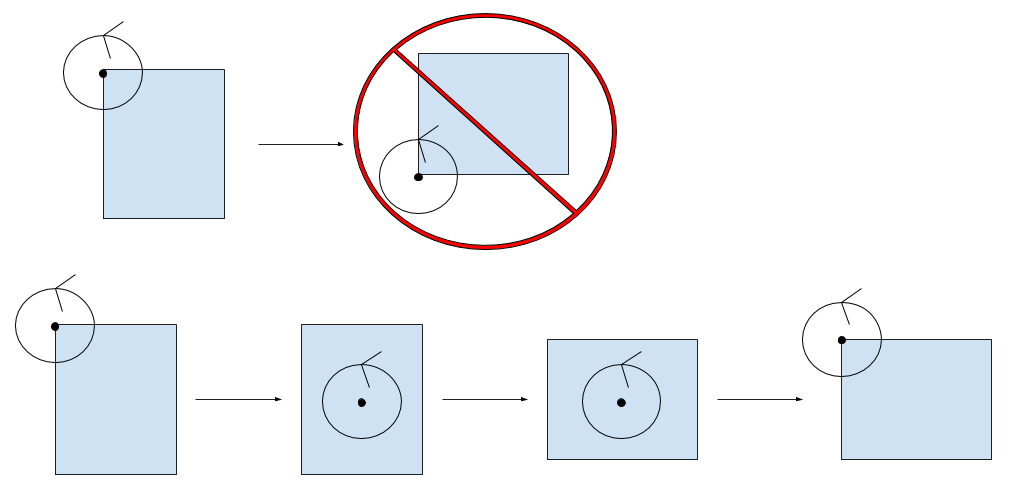
\includegraphics[scale=0.4]{Rotation.png}
	\caption{Rotation process for objects}
	\label{fig:rotation}
\end{center}
\end{figure}

\newpage

\section{Position Recordings}
\label{sec:positionrecordings}
As we mention in the prelude to \textit{Chapter \ref{cha:sysdesign}}, one of the limitations for this project was that we do not to record videos coupled with geo-tags to use with our interface. This is a common feature with photos, as many cameras supports including geo-tags within a .jpg file's exif-data. Recently smartphones has actually come to support geo-tagging videos as well, but this video geo-tagging process is not done in the same way as with photos. As of this paper there is no standard for geo-tagging videos. When recording videos with Android OS geo-tags are not stored with the actual video itself, but with an additional log file tied to the video. For iOS the geo-tags \textit{are} stored within the video's QuickTime metadata. In our case, as we were using Android, we would have had to implement support for these log files within our interface to be able to fetch the coordinates for the recorded videos. This would however not be a general solution as it would not have worked with recordings made with other systems than Android. In the future a standard for geo-tagging videos might exist, allowing for an easier implementation of these kind of geo-tagged recordings into our interface and others. 

There is also the case of fetching a continuous stream of coordinates from a live video stream. Our interface could be made to support several live recorded streams, each with a dynamic coordinate which regularly updates its geographical position and angle on our interface's geographical map. As all of the common recording softwares with video geo-tagging we know of only support including a single static geographical position with a recorded video, such a recording software would have to be developed.

\section{GPS \& Sensors}
\label{sec:gpsandsensors}
As we have already made clear, our interface make use of two different location based inputs to accurately draw positions of the recordings onto the interface’s geo-based map. These are the GPS-coordinates and the angles used of the recording units. While we synthetically generated these coordinates and angles to prove the functionality of the interface, there are of course autonomous means of collecting these datas using GPS-receiver and some other device sensors which we will elaborate on here. Namely, the magnetometer and gyroscope.

\subsection{Collecting Position Data}
\label{sec:collectingpositiondata}
One of the reasons we synthetically generated the coordinates of our recording locations done for the interface’s tests in this report was that the position determining provided by our devices’ GPS was not accurate enough. As the recording area for our test case was pretty small we wanted a high accuracy for our recording positions. 

GPS for civilians and consumer, also called Standard Positioning System (SPS), used today provide users with a range error of about 3 meter in the best case scenario with a well designed receiver, or an accuracy of up to a 7.8 meter deviation 95 \% of the time \cite{spsperf}. However, expanding GPS services are constantly a process in work and there are new standards being developed by the U.S. Air Force which will be available for consumers in the near future, namely L1C, L2C and L5. Among these is L2C, the modernized GPS signal standard, targeted for consumer use. The main cause of inaccuracy in today’s L1 C/A standard is called ionospheric delay, which basically is a delay that arises from atmospheric conditions and affects the speed of the GPS-signals and the resulting accuracy of the positioning system. The L2C standard seeks to resolve this using ionospheric correction to measure and therefore remove the delay to further boost the position determining accuracy.\cite{gpsdir} Recent tests show that the new L2C standard provides a ~0.5 meter average in user range error, which is a significant improvement to the previous standard\footnote{CNAV Performance: http://www.navcen.uscg.gov/?pageName=CNAV$\_$Performance}.

All in all, the current state of GPS technology would have to make do if one were to autonomously measure position data for recordings to input into our geographical interface today. There are also cases where GPS would not function at all, like if the recordings were done indoors for the interface where GPS signals can not reach. What could act as a substitute for GPS in these cases is mentioned in \textit{Section \ref{sec:phoneapi}}.

\subsection{Collecting Rotational Data}
\label{sec:collectingrotationaldata}
Secondly, we also synthetically generated the angles used for the interface in this report. Our interface accepts an angle relative to the north cardinal direction and points the arrow representing a video stream in that direction. The most obvious way of collecting this data through devices would be to use a compass made up by a magnetometer built into the recording device, but we found that the compasses in our phones were pretty inaccurate. The reason for this might be because the magnetometer is heavily dependant on its calibration and need relatively frequent recalibration to maintain its accuracy and also because of electromagnetic interference from other nearby electronic devices. We discussed this and came up with an idea that might solve the issue.

With a recent calibration of the magnetometer one can get a good approximation of the bearing of the device. The issue here is maintaining this accuracy when turning the recording device, because of the sloppy nature of the magnetometer sensor. Many mobile devices nowadays are equipped with a gyrometer with the main purpose of tracking the device’s orientation. The gyrometer does a way better job of keeping track of the device’s orientation than that of the magnetometer, because its measures are only dependent on itself and the static gravitational field rather than its surrounding magnetic field. We thought of a solution in which a client would initially synchronise the recently calibrated magnetometer with the gyrometer, as in the gyrometer is initially given the magnetic heading which it will keep track of when the device deviates from its original orientation and position. This would allow the device to return its rotation relative to the north cardinal direction even snappier and independently of any eventual electromagnetic interference or distortion. 

\subsection{Phone API}
\label{sec:phoneapi}
Most mobile devices today use an application programming interface (API) that allows for a client to get current geographical location and compass directions. Most smartphones has a compass API that allows to get direction information relative to the cardinal directions with the help of the sensors built into the phone. Since our geo-based interface accepts geo-location and direction information it would be great if there was an API that could allow us to retrieve geographical location and direction and tag videos autonomously. There exists an API called W3C Geolocation API that is used for retrieving geographical location information for a client-side device (e.g. smartphone) \cite{geoapi}. The API uses multiple sources to get the location of the device with a high accuracy. Example of sources are: Wi-Fi, Radio Frequency Identification (RFID), GSM/CDMA, GPS etc. The API is used for defining high-level interface to location information associated with the client device. Even though it is an API that retrieves a geographical position for the client device it also takes privacy into account, allowing a user to choose if they want to share their location to a remote web server \cite{useofgeo}. There have been works that have looked at ways of improving the framework regarding privacy issues for W3C \cite{privacyissues}. Since location information can be a sort of sensitive information for many people it is good if the API is supported to an extend where privacy is taken into account. The W3C also has an API called W3C Compass API that combined with the Geolocation API allow for retrieving geographical and directional information \cite{compassapi}. There also exist something called Adobe PhoneGap Build\footnote{Adobe PhoneGap Build for combining compass data with HTML-based applications: https://helpx.adobe.com/phonegap-build/how-to/phonegap-compass-api.html} (Bd) that allows to combine a mobile’s compass sensor with a HTML-based application. This service can be used to allow for building our geo-based media player for smartphones and allow to retrieve compass data with the help of the Compass API.

Tagging user-created content with a location is something that is wanted for our application, and embedding it onto the recording itself would have been ideal. A general idea to do this is by getting the geo-location information when the user initially starts its recording, or by collecting the geographical data live during a whole stream or a specific time of an event depending on the resulting accuracy. \cite{locationstrategies}

\subsection{VR Technology}
\label{vrtechnology}
Virtual Reality (VR) is a new and exciting jump in technology and it offers new ways of educational learning for people and to be entertained. It also offers ideas and techniques that can be used for other things as well, and in the case with our interface potentially improve the compass for a phone which is needed for future work if our media player would be further expanded upon to work with recordings done by compass equipped smartphones. It could improve the accuracy of the smartphones compass and also allowing for potentially automatic retrieval of geographical position and direction to be more accurate. 

There are as of this paper three major Virtual Reality Headsets on the market; Playstation VR, Oculus Rift and HTC Vive. Other companies like Samsung has also started developing their own VR-headset. This is something new and exciting for the industry and is a milestone in technology regarding sensor usage for head and movement tracking. The technology is very interesting in the way that VR-headsets keep track of a user's movements and direction. Oculus Rift uses a tracking system called Constellation\footnote{Constellation: http://xinreality.com/wiki/Constellation}. It utilizes optical sensors that that can detect IR LED markers on their devices and features 360 degree tracking. In addition to Constellation the Oculus Rift uses something called IMUs\footnote{IMU: http://xinreality.com/wiki/IMU} as its primary tracking device. It is an electrical sensor composed of accelerometers, gyroscope and magnetometers. What is common among all the three big VR-headsets is that they use gyroscope and accelerometers sensors, where gyroscope is for orientational tracking and accelerometer is for velocity tracking. They also has something called a 6 degree of freedom (6DOF) rotational and position tracking which for the Oculus Rift is performed by the Constellation. This is basically six possible motions that the headset can recognize.

All three VR-headsets are similar but not entirely similar, they all allow for a user-friendly experience with a high quality and even if the ideas for motion tracking can seem identical they all do something a bit differently in-order to allow for the best experience. The ideas with using gyroscope is something we figured would be the most important thing to look at for keeping track of the orientational movement for the device as described earlier. Accelerometer is not as important for us since we do not care about keeping track of the velocity in movements.

\section{The Test Case}
\label{sec:test case} 
For our test case, there is one thing we in hindsight would have changed if we would have redone it. In our case we set up only two cameras at a time to get multiple views of what was happening at the scene from different locations, simultaneously. To further and better prove the functionality of our user interface in a test case, we should have brought some more volunteers and cameras along with us to get even more point of views of the same scene at one point in time. While doing two recordings at once was enough to prove the functionality of this feature, more recordings would have been a beneficial addition. 

Another thing that could have been done differently is to have made more tests when looking at consistency when switching between different videos on-demand. However, 200 video swaps is more than enough to give a general idea of how long it takes to switch between a video but more tests could have been done to check where the most time consuming place is. For example, the time it takes to load a video from the Adobe Media Server 5 may have taken the longest or when retrieving a video from the plug-in script.

\section{Adobe Flash}
\label{sec:adobe flash}

Furthermore, as mentioned previously in this report, Adobe Flash is becoming more deprecated by the day even by Adobe themselves. Because of this, if the project was redone the interface would be better suited to be implemented in the media player built from a more modern alternative such as Flash's main competitor, or rather replacement, HTML5.

\section{Issues with the Server}
\label{sec:serverissues}

One big obstacle which unnecessarily cost a lot of time was setting up the server we used. Initially we used something called a WAMP\footnote{WAMPSERVER: http://www.wampserver.com/en/} server at the start of the project which enabled us to stream videos using HTTP through an Apache HTTP Server. However, since idea of prefetching was still present at that point of the project there was a need to switch to Adobe Media Server 5 since it would allow us to stream chunked bits of video used for the prefetching. While setting up the servers we ran across numerous problems with different kinds of security errors which would not allow us to stream the videos using HTTP. While trying to solve these issues we found that since the Apache server ran on a Windows 10 client there was a process that blocked the server that was needed to be stopped\footnote{For Windows 10 use the following command to stop the process blocking Apache: iisreset /stop}. Only then was the server able to run and allow videos to be streamed with HTTP.

\section{Project Structure Improvements}
\label{sec:psi}

If the project was redone we would have made a more definite time plan of what was needed to be done. Our time plan, even though straightforward, was not very detailed. We knew what we wanted to accomplish and when but we did not really know how we would go about to accomplish it. This ended up unnecessarily consuming a lot of time since we did not know where to look in the giant web of provided code to solve any eventual issues or where exactly to implement the changes and solutions. When we worked on this project we needed to ask for a lot of help from our supervisor in order to know where to look before coding. What we could have done instead is make a time plan that we later could showed to our supervisor and then asked how we could go about to accomplish it. It could also have been very helpful if we could have been provided with some feedback on the time plan by our supervisors to know it it was any good or if it could have been improved in some way. 

\section{Work in a Wider Context}
\label{sec:workinawidercontext}
While the purpose of our proof-of-concept has proved successful, there are of course means to further extend on our work and develop further functionality into the interface. One example of an extension would be to implement support of omnidirectional cameras. The main purpose of the project's interface is to allow the user to view the same area from multiple, preferably as many as possible, different locations and angles. Because of this an upgrade from standard cameras with a regular field of view to omnidirectional cameras would be a natural upgrade to give the user an even better overview of the recorded area. This would change the purpose of the interface to allowing the user to view the same area from multiple locations and \textit{all} of the locations' angles.

Another video player, YouTube, already has omnidirectional camera support today\footnote{A Youtube creator blog about the 360$^{\circ}$ camera feature: https://youtubecreator.blogspot.se/2015/03/a-new-way-to-see-and-share-your-world.html, Fetched: 2016-05-19} with a feature Google calls \textit{360-degree videos}. As we mention an eventual support of omnidirectional recordings for our interface, we think an implementation much like YouTube's would be suitable for this purpose. However, YouTube lacks the support of multiple recordings and the option to swap between them. With this said a refined version of our interface could further contribute to media players like YouTube's and many others. The usefulness of the interface would also not have to be limited to entertainment streams. A news outlet could also make use of the interface by recording a scoop, perhaps live, from different positions in which news-reader could select a specifically located stream from the media's web page's media player.

When looking at studies about 360$^{\circ}$ cameras there was a work that looked at viewing meetings with the help of different cameras and equipments \cite{distributedmeetings}. They looked at a way for a person that could not attend a meeting to view the meeting, during or after the meeting, with a rich and enjoyable experience. By providing a system called Distributed Meetings (DM), they are able to broadcast and record meetings with various devices and cameras. When viewing a pre-recorded meeting the system allows on-demand viewers with indexes of a whiteboard content and speakers to allow for users to choose a video to only show specific parts \cite{distributedmeetings}. Our work can help enhance this experience in the context of allowing for a better and interactable meeting experience. Allowing users to switch between recording cameras in an intuitive and, in the future, seamless way. This would make interaction more enjoyable and better for the users to make the user a greater part of the meeting even though they are far from the meeting.

Some other interesting works have dwelved more into how to prefetch in an effective way \cite{watchingprefetching, tvservices}. Khemmarat et al. \cite{watchingprefetching} have looked at different ways to prefetch videos in-order to allow for the best user experience. While watching a Youtube video, the user experience is significantly increased when the time the video is paused and buffering is minimal. They provide an approach that tries to predict which video a user will click and and prefetch it. By looking at three different schemes they found that by combining caching and prefetching the hit-ratio, for which a clicked video is pre-buffered, would increase up to 80 \%. Their proposed schemes improves video playback in a way that it avoids playback delay. The trade-off of a higher bandwidth usage is minimized when combining prefetching and caching of videos \cite{watchingprefetching, tvservices} and by not having large amount of videos to prefetch \cite{watchingprefetching}. If this were to be combined in some way with what we want to accomplish with prefetching then it will allow for a much better video experience.
